\chapter{Taylor Series}
\label{chtaylor}

Polynomials are in many ways the easiest, most convenient, functions to
work with, and it thus would be nice if every function was a polynomial. The
formula for the geometric series shows that this might be possible, if we
allow for something like a polynomial, but of infinite degree:
Consider the function $f(x)=1/(1-x)$, that is not a polynomial. Then, as
long as $\sz{x}<1$ we have that
\[
\frac{1}{1-x}=1+x+x^2+x^3+\cdots=\sum_{i\ge 0} x^i
\]
(by the summation formula for the geometric series).

In this chapter we will work with three ideas: The first is how we can
approximate any function by a polynomial (called a Taylor polynomial), and to see that such
approximations become better as the degree increases.
The second topic is what a polynomial of infinite degree should be (it will
be called a power series). Finally we will extend Taylor polynomials to
infinite degree to see how we can represent most of the functions that we
encounter as power series.

\section{Taylor Polynomials}

The basic idea for finding a polynomial approximation of a function is that
we want the polynomial and the function to have the same values at a point,
as well as the same values of the derivatives.\mynote{We shall see that this
turns out to be a useful approach. In fact it is better than the alternative
approach of having the same values at a number of different points.}

We start by considering values at $0$ and consider a polynomial
\[
p(x)=a_0+a_1x+a_2x^2+\cdots+a_nx^n=\sum_{i=0}^n a_i x^i
\]
Its derivatives are
\begin{eqnarray*}
p'(x)&=&a_1+2a_2x+3a_3x^2+\cdots+n\cdot a_nx^{n-1}=\sum_{i=1}^n i\cdot a_i x^{i-1},\\
p^{\prime\prime}(x)&=&1\cdot 2a_2+2\cdot 3a_3x+\cdots+(n-1)\cdot n\cdot
a_nx^{n-2}=\sum_{i=2}^n (i-1)i\cdot a_i x^{i-2},\\
&&\mbox{and generally, for the $k$-th derivative }\\
p^{(k)}(x)&=&\sum_{i=k}^n (i-k+1)\cdots(i-1)i\cdot a_i x^{i-k}.\\
\end{eqnarray*}
This means that the value of this derivative at $0$ is the constant term
(for $i=k$):
\[
p^{(k)}(0)=1\cdot2\cdots(k-1)\cdot k a_k=k! a_k,
\]
where $k!$ (called $k$-\defini{factorial}) is the product over all numbers
from $1$ to $k$.
\smallskip

To ensure that the derivatives of $p(x)$ are equal to those of $f(x)$, we
thus get the conditions $f^{(k)}(0)=k! a_k$ which we can solve for
\[
a_k=\frac{f^{(k)}(0)}{k!}.
\]
\begin{defn}
Let $f\colon\R\to\R$ be a function that is repeatedly differentiable.
The \defini{Taylor polynomial}
for $f$ around $a=0$ of degree $n$ is the polynomial
\[
\sum_{i=0}^n\frac{f^{(i)}(0)}{i!} x^i
\]
(where $f^{(k)}(0)$ is the value of the $k$-th derivative at $0$).
\end{defn}
For example, if $f(x)=\exp(x)=e^x$ (we pick this example for the easy pattern of
derivatives), we have that
\[
f(0)=e^{(0)}=1,\quad
f'(0)=e^{(0)}=1,\quad
f^{\prime\prime}(0)=e^{(0)}=1,\quad\ldots,
f^{(k)}(0)=e^{(0)}=1
\]
and we thus get the Taylor polynomials of degree $0,1,2,3,\ldots$ as
\begin{eqnarray*}
p_0(x)&=&\frac{1}{0!}x^0=1\\
p_1(x)&=&\frac{1}{0!}x^0+\frac{1}{1!}x=1+x\\
p_2(x)&=&1+x+\frac{1}{2!}x^2=1+x+\frac{x^2}{2}\\
p_3(x)&=&1+x+\frac{x^2}{2}+\frac{1}{3!}x^3=1+x+x^2+\frac{x^3}{6}\\
p_4(x)&=&1+x+\frac{x^2}{2}+\frac{x^3}{6}+\frac{x^4}{24}\\
&\vdots&\\
p_n(x)&=&\sum_{i=0}^n \frac{x^i}{i!}
\end{eqnarray*}
The first few polynomials, together with the function $f(x)=\exp(x)$ are
shown in Figure~\ref{figtayexp}.
\begin{figure}
\begin{center}
%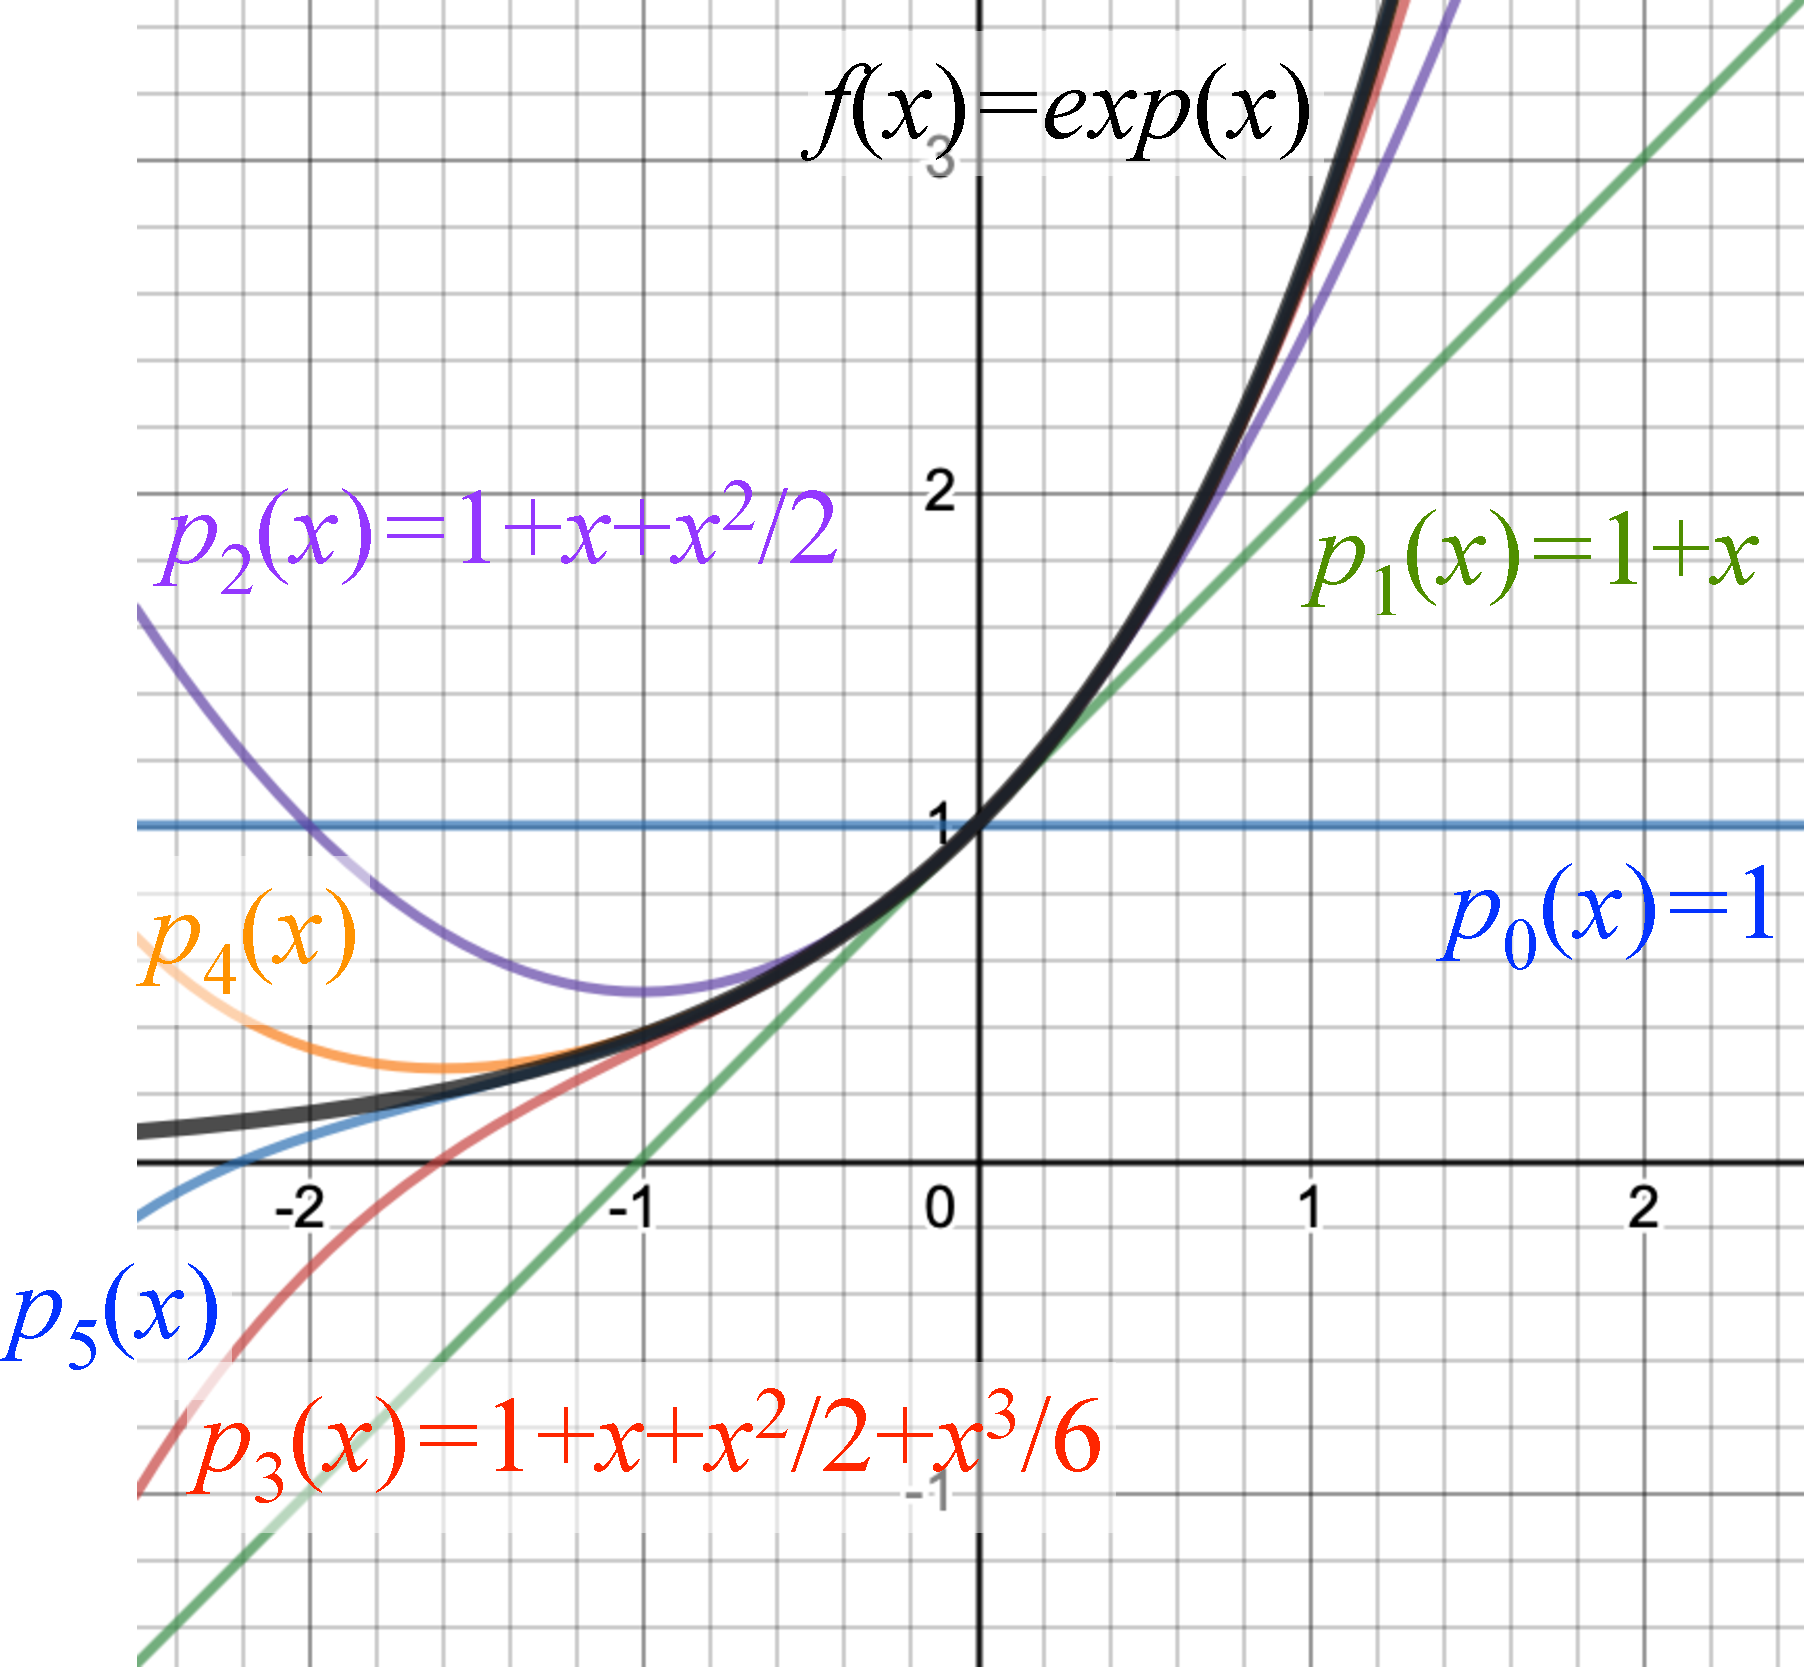
\includegraphics[width=6cm]{pic/TaylorExp.pdf}
\anngraphics{6cm}{pic/TaylorExp.pdf}{The first five Taylor approximations
for $f(x)=e^x$ are graphed on a coordinate plane. All intersect the point
$(0,1)$, but have varying degrees of curvature. As the $k$ value of the
Taylor approximation increases, the graph more closely conforms to the graph
of $f(x)=e^x$.}
\end{center}
\caption{Taylor approximations to $\exp(x)$}
\label{figtayexp}
\end{figure}


If we choose instead
$f(x)=\frac{1}{x+2}$, we get
\begin{eqnarray*}
f'(x)&=&-\frac{1}{(x+2)^2}\\
f^{\prime\prime}(x)&=&\frac{2}{(x+2)^3}\\
f^{\prime\prime\prime}(x)&=&-\frac{6}{(x+2)^4}\\
f^{(k)}(x)&=&(-1)^k\frac{k!}{(x+2)^{k+1}}\\
\end{eqnarray*}
and thus Taylor polynomials
\begin{eqnarray*}
p_0(x)&=&\frac{1}{2}\\
p_1(x)&=&\frac{1}{2}-\frac{x}{4}\\
p_2(x)&=&\frac{1}{2}-\frac{x}{4}+\frac{x^2}{8}\\
&\vdots&\\
p_5(x)&=&\frac{1}{2}-\frac{x}{4}+\frac{x^2}{8}-\frac{x^3}{16}+\frac{x^4}{32}-\frac{x^5}{64}
\end{eqnarray*}
These polynomials are shown in Figure~\ref{figtayoneo}.
\begin{figure}
\begin{center}
%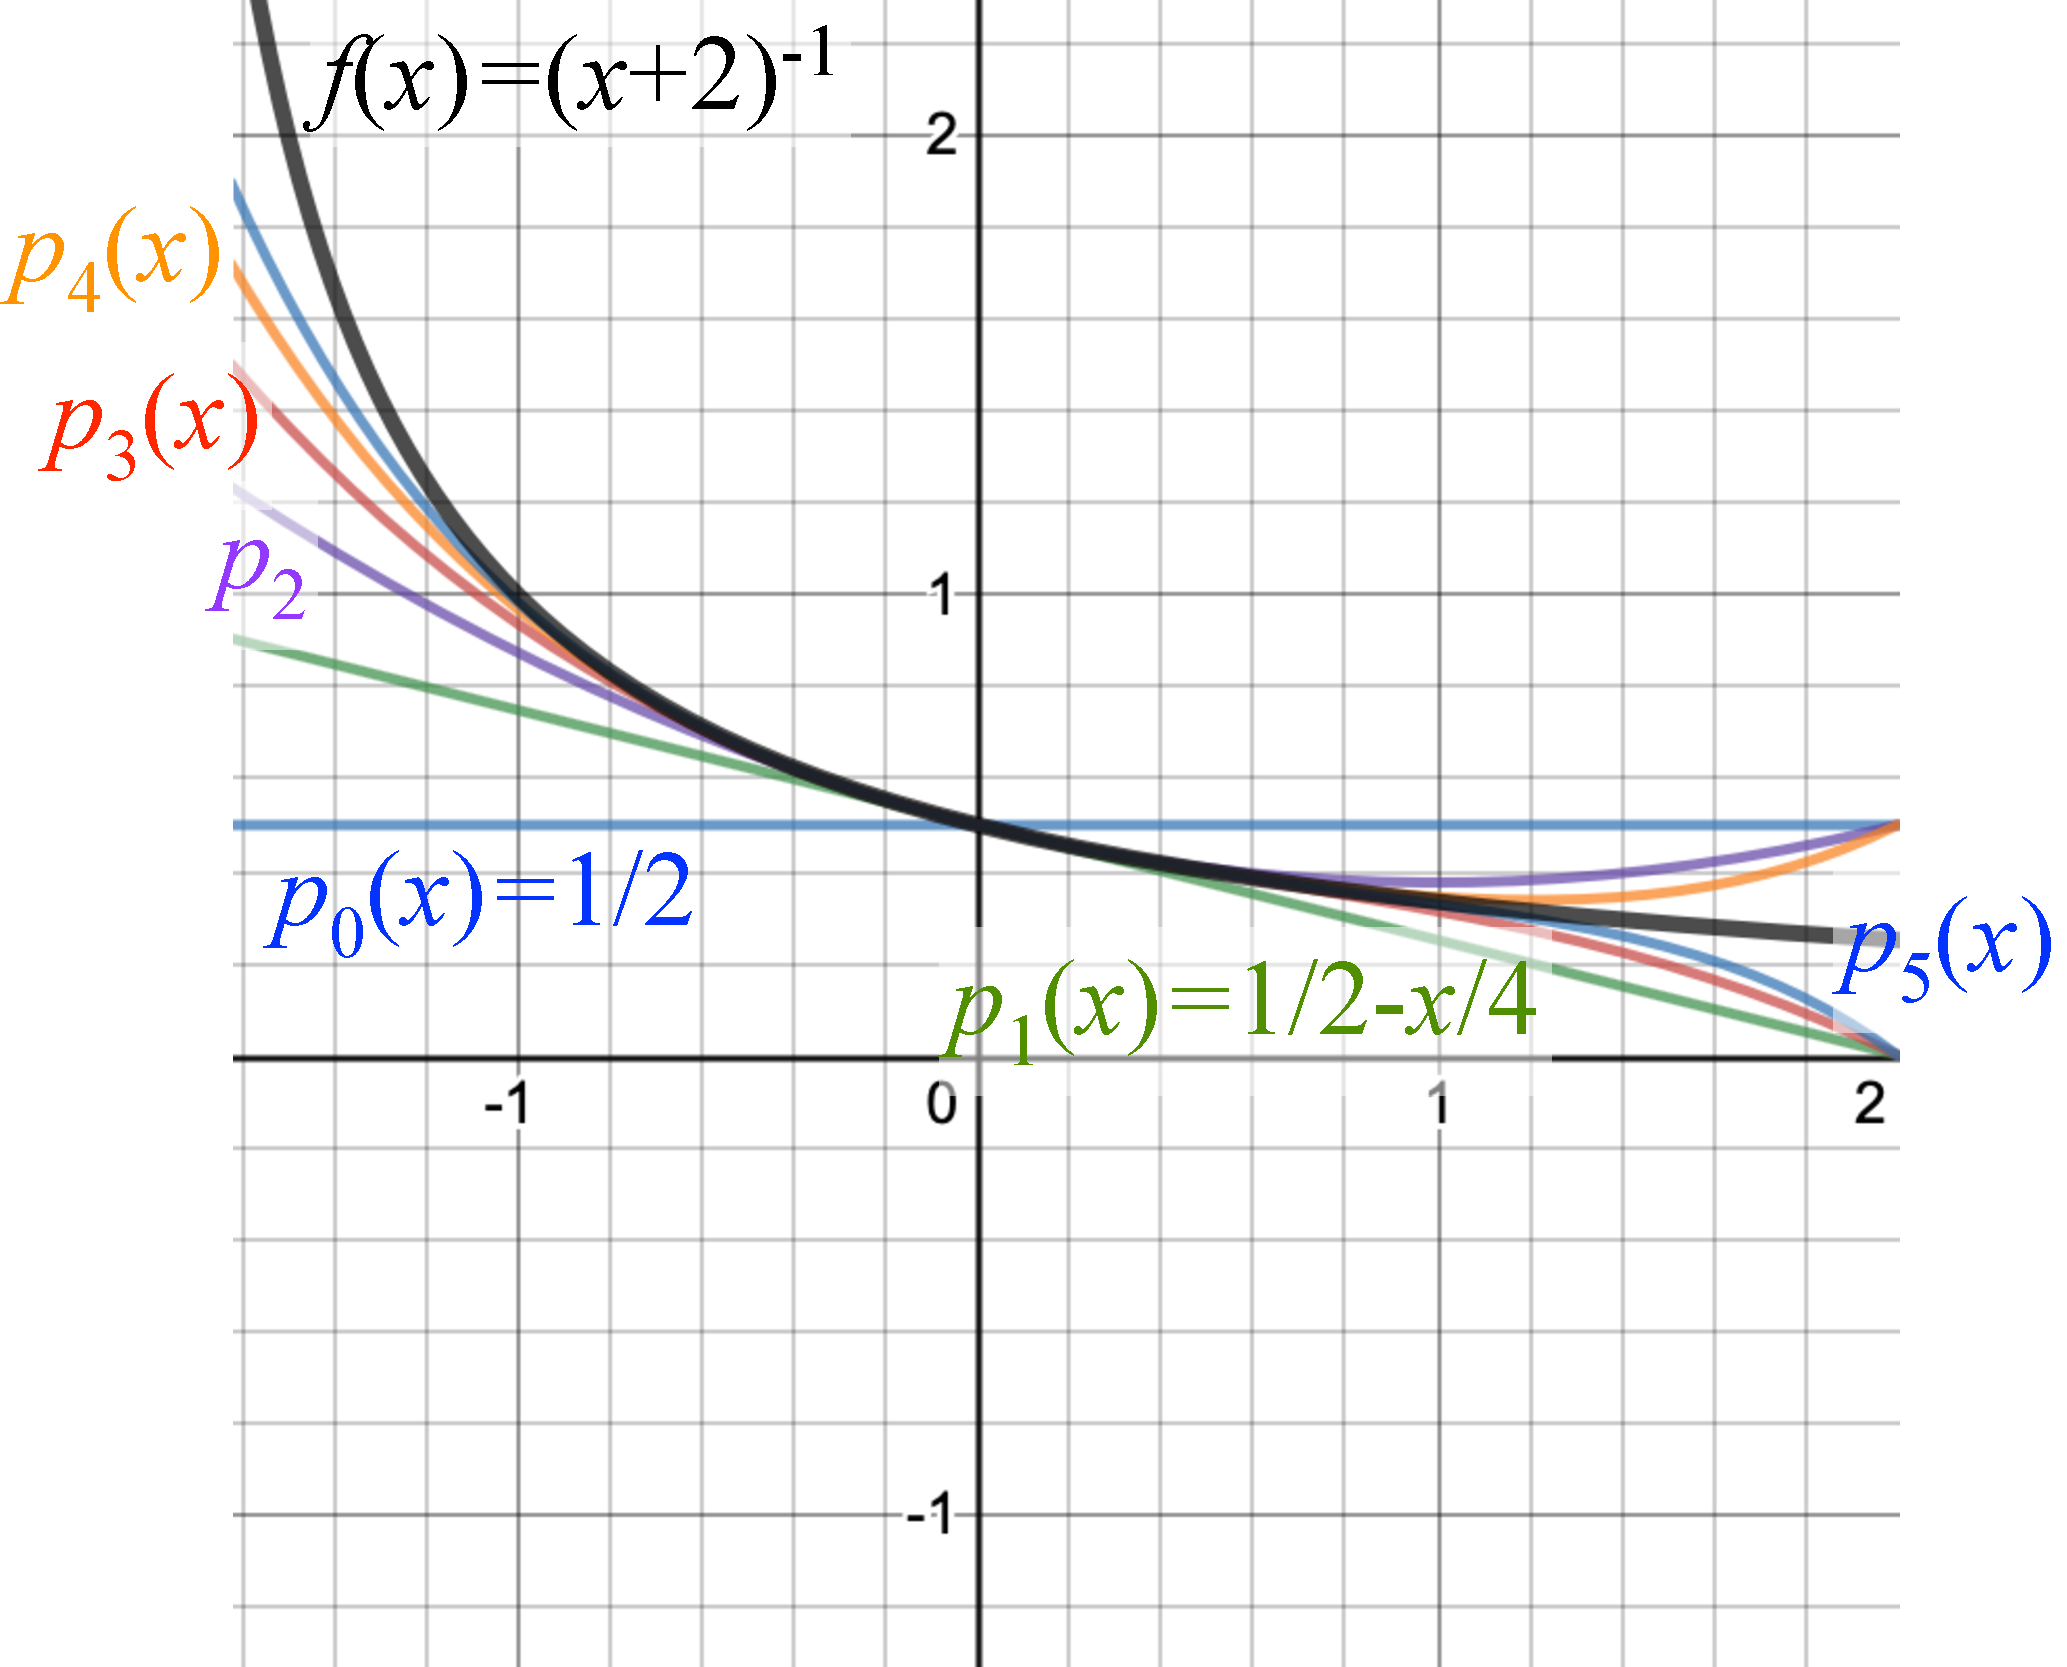
\includegraphics[width=6cm]{pic/TaylorOneOverxP2.pdf}
\anngraphics{6cm}{pic/TaylorOneOverxP2.pdf}{The first five Taylor
approximations for $f(x)=(x+2)^{-1}$ are graphed on a coordinate plane.
Again we see that as the $k$ value of the Taylor approximation increases,
the graph of the approximation more closely comforms to the graph of
$f(x)=(x+2)^{-1}$.}
\end{center}
\caption{Taylor approximations to $(x+2)^{-1}$}
\label{figtayoneo}
\end{figure}


Finally, take $f(x)=\sin(x)$, and we get
\[
f(0)=\sin(0)=0, f'(0)=\cos(0)=1,
f^{\prime\prime}(0)=-\sin(0)=0,
f^{\prime\prime\prime}(0)=-\cos(0)=-1,\ldots
\]
Thus every second coefficient is zero and we get new Taylor polynomials only
for odd indices:
\begin{eqnarray*}
p_1(x)=p_2(x)&=&x\\
p_3(x)=p_4(x)&=&x-x^3/6\\
p_5(x)=p_6(x)&=&x-x^3/6+x^5/120\\
\end{eqnarray*}
as shown in Figure~\ref{figtaysin}.
\begin{figure}
\begin{center}
%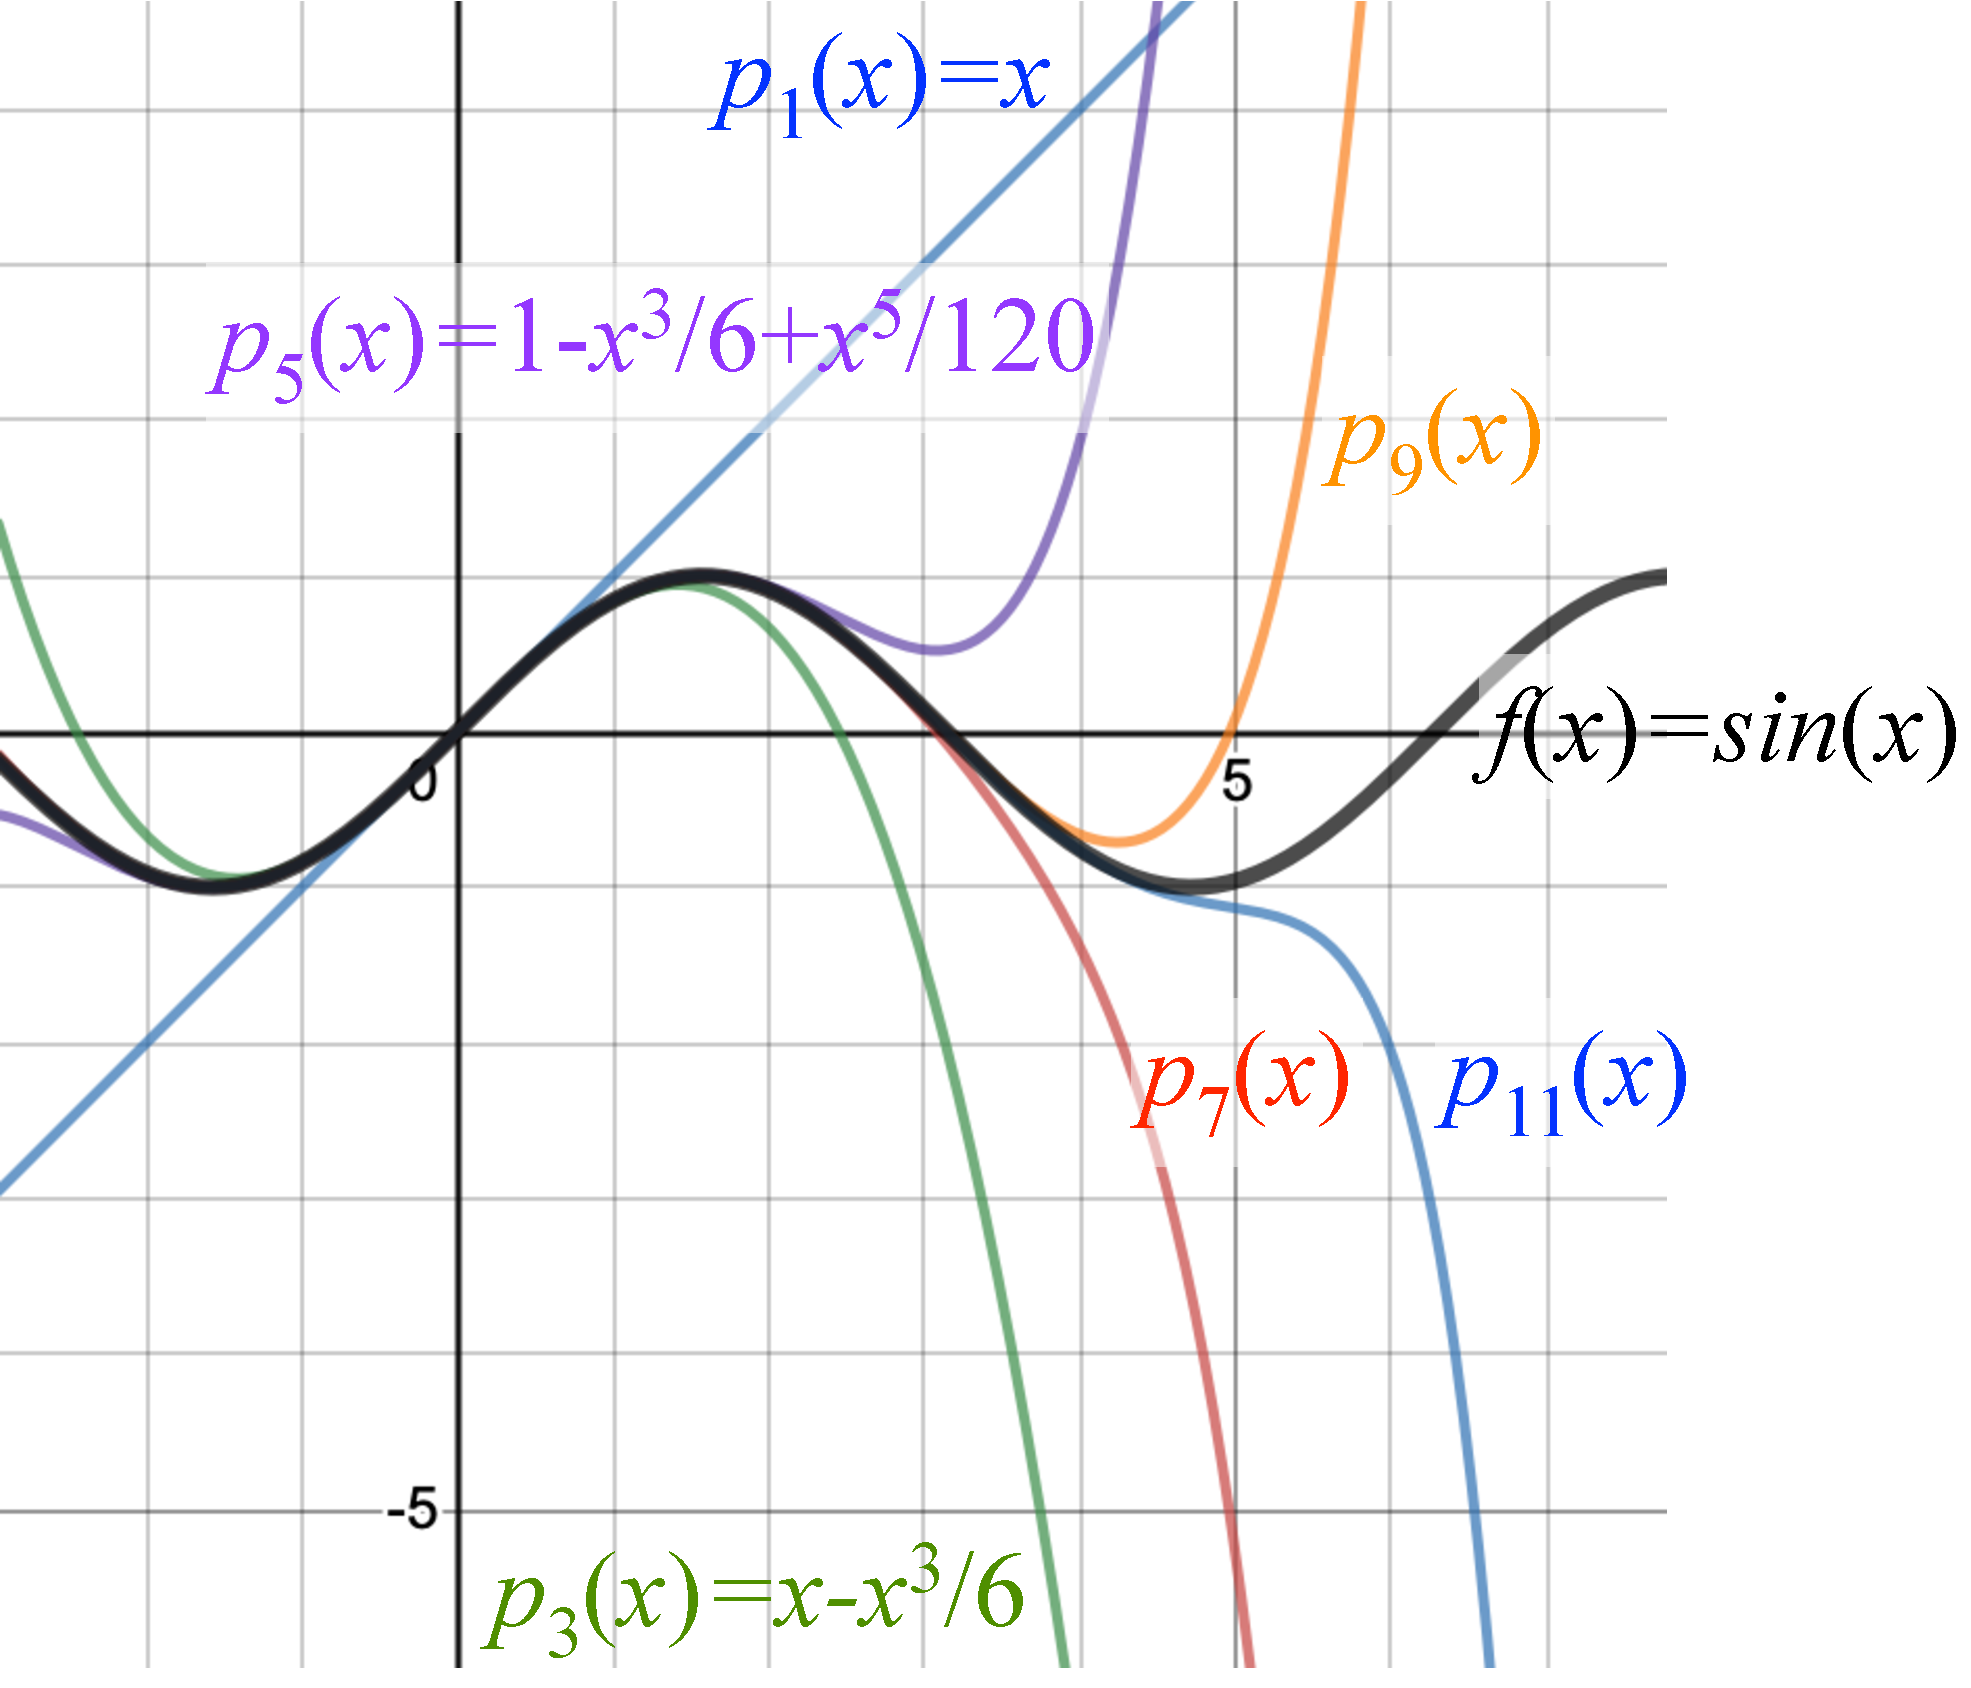
\includegraphics[width=6cm]{pic/TaylorSin.pdf}
\anngraphics{6cm}{pic/TaylorSin.pdf}{Several Taylor approximations for
$f(x)=sin(x)$ are graphed on a coordinate plane, including those of degree
7, 9, and 11. }
\end{center}
\caption{Taylor approximations to $\sin(x)$}
\label{figtaysin}
\end{figure}
These calculations allow us to make the following observations:
\begin{enumerate}
\item As the degrees increase, Taylor polynomials just accumulate further
terms.
\item The Taylor polynomials approximate well around $a=0$, but the
approximation becomes worse if we go away from $a=0$.
\item The approximation gets better, the higher the degree of the Taylor
polynomial is.
\end{enumerate}
We shall give a justification for this (and show that this true in general)
below.
\bigskip

So far we have formed Taylor polynomials around $a=0$. The rules we know
about shifting functions horizontally allow us to define a polynomial around
arbitrary real numbers $a$ by shifting accordingly. The corresponding (more
general) definition is unsurprising.
\begin{defn}
Let $f\colon\R\to\R$ be a function that is repeatedly differentiable
and $a\in\R$.
The Taylor polynomial for $f$ around $a$ of degree $n$ is the polynomial
\[
\sum_{i=0}^n\frac{f^{(i)}(a)}{i!} (x-a)^i
\]
(where $f^{(k)}(a)$ is the value of the $k$-th derivative at $a$). We call $a$
the \defini{center} of the Taylor polynomial.
\end{defn}
Note that for $a=0$ this just gives the prior definition.

For example, using the calculations of the derivatives we already did, 
we find the Taylor
polynomial of degree $5$ for $f(x)=\frac{1}{x+2}$ around $x=-1$ as
\[
1-(x+1)+(x+1)^2-(x+1)^3+(x+1)^4-(x+1)^5.
\]
Figure~\ref{figtayoneoplus} compares this Taylor polynomial with the one
around $a=0$ we had computed above. Unsurprisingly the polynomial around
$a=-1$ approximates better for $x$-values closer to $-1$, while the one
around $a=0$ approximates better for $x$-values closer to $0$.
\begin{figure}
\begin{center}
%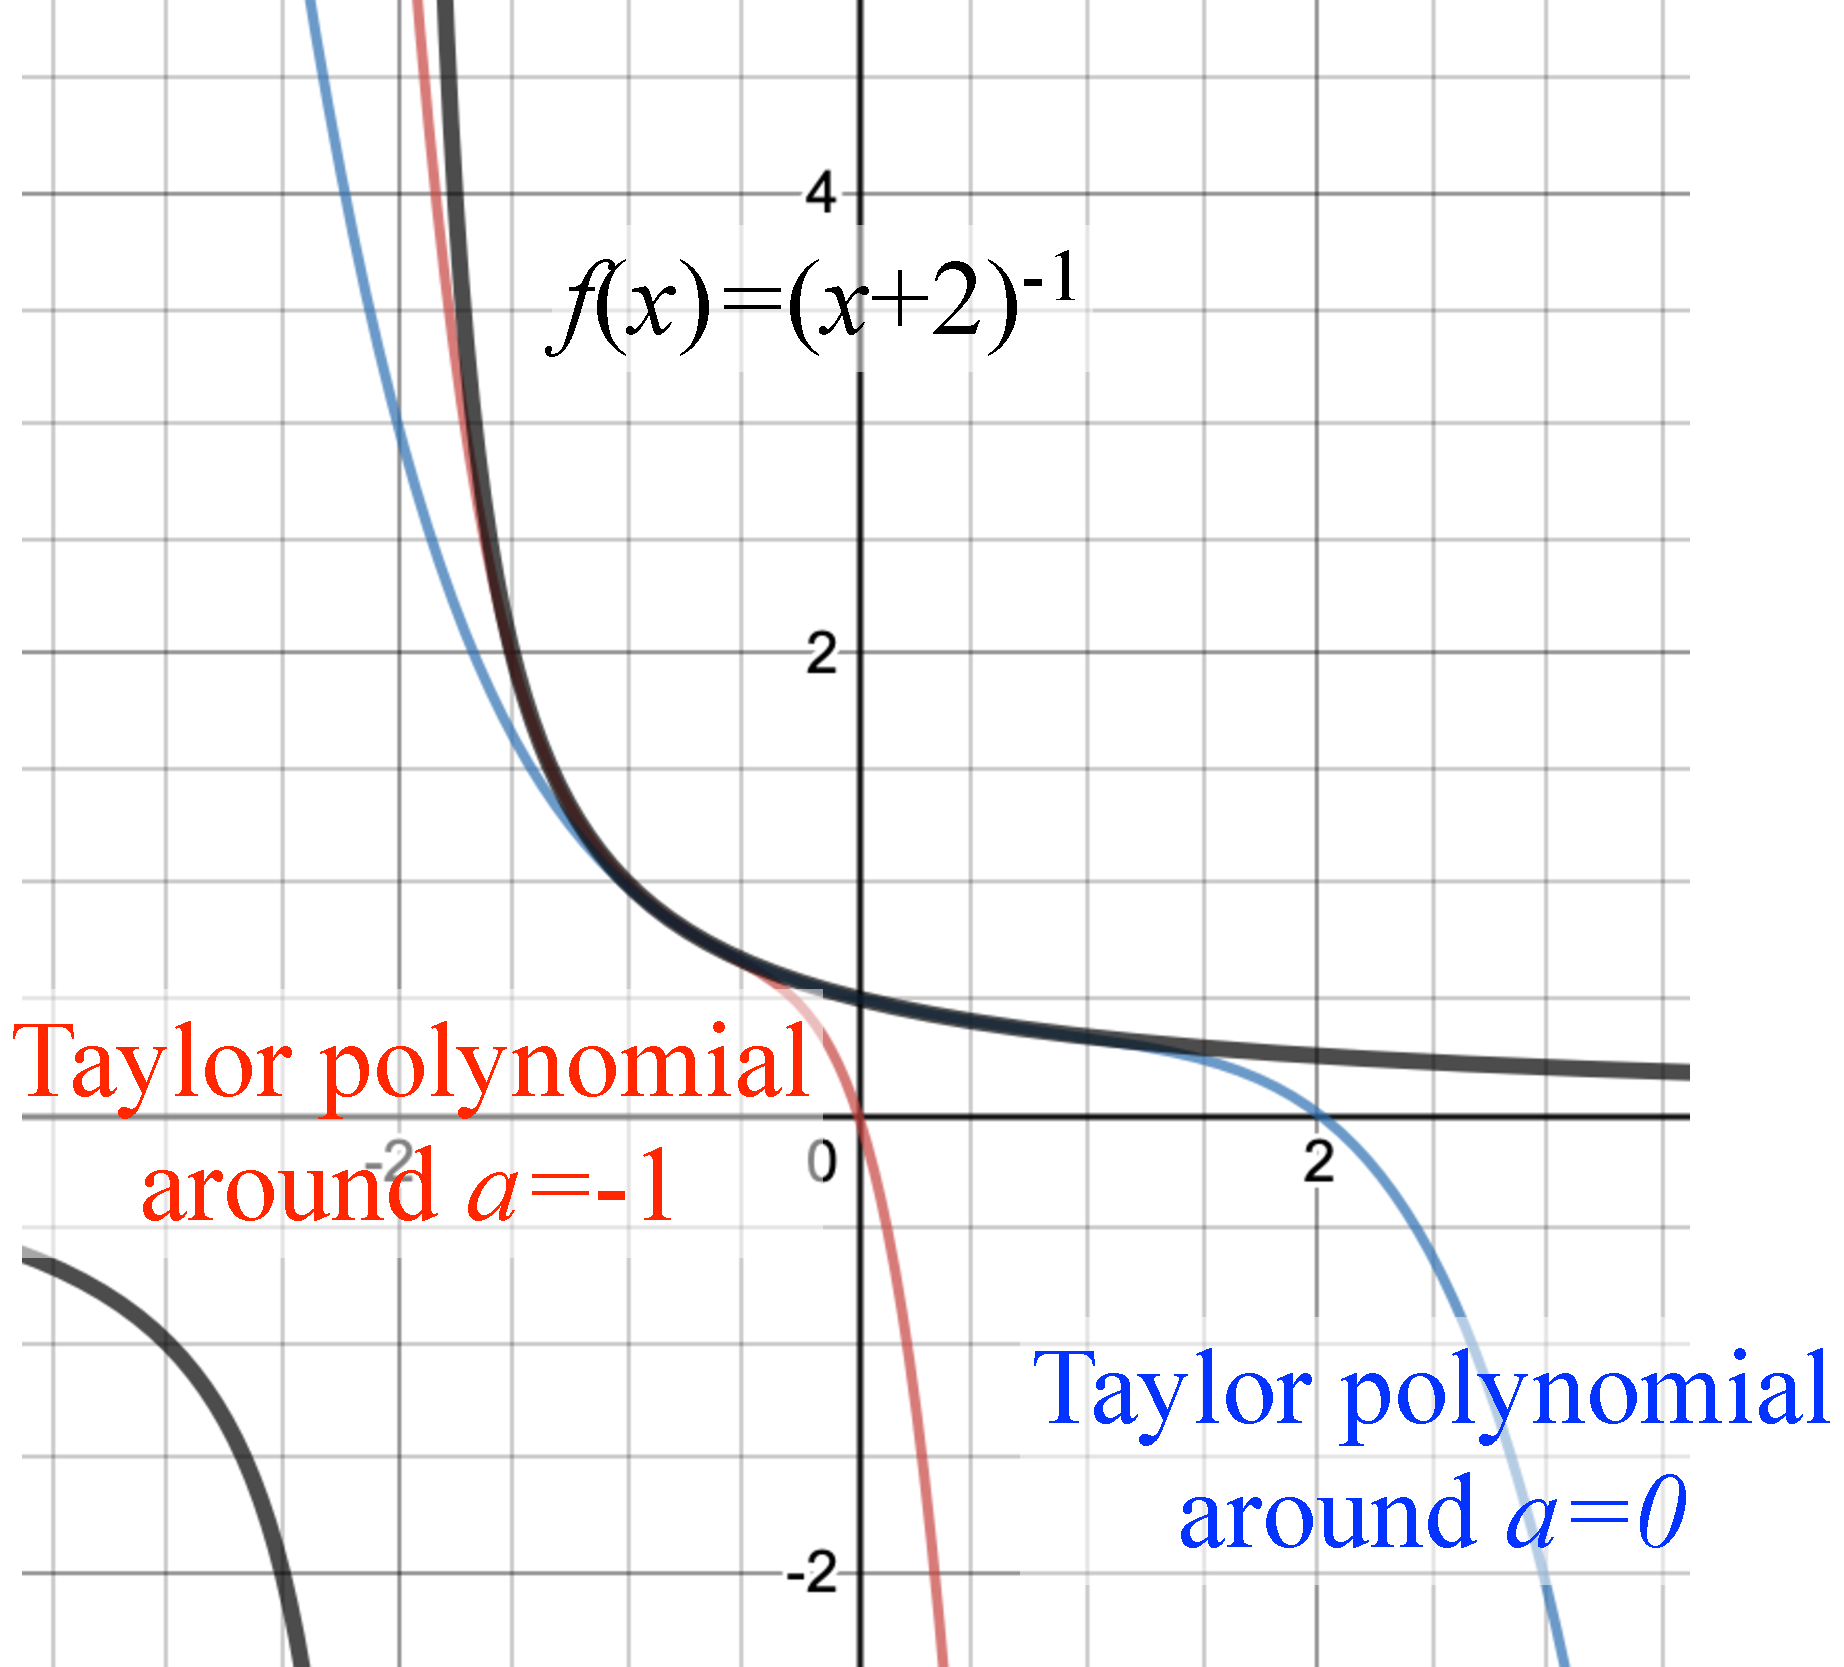
\includegraphics[width=6cm]{pic/TaylorOneOverxP2Plus.pdf}
\anngraphics{6cm}{pic/TaylorOneOverxP2Plus.pdf}{The graph of
$f(x)=(x+2)^{-1}$ is plotted on a coordinated plane with a Taylor polynomial
centered at $a=0$ and a Taylor polynomial centered at $a=-1$. We see that
the Taylor polynomials approximate well near the center, but less well
further away.}
\end{center}
\caption{Taylor approximations to $(x+2)^{-1}$ around $a=-1$ and $a=0$}
\label{figtayoneoplus}
\end{figure}

\subsection{Approximation Error}

The core to understanding the way a Taylor polynomial approximates a
function is the \defini{error term}. One can show:
\begin{thm}
Let $f\colon\R\to\R$ be  a function that can be differentiated $n$ times,
$a\in\R$, and $l>0$.
Then the approximation error of the Taylor polynomial of degree $n$ for
$x$ in in an interval of length $2l$, centered at $a$ (that is,
$\sz{x-a}\le l$, equivalently $a-l\le x\le a+l$) is:
\[
\sz{f(x)-p_n(x)}\le \frac{M}{(n+1)!}\sz{x-a}^{n+1}\le \frac{M}{(n+1)!}l^{n+1}
\]
where $M$ is an upper bound for the value of the $n+1$-st derivative of $f$
on the interval $a-l\le x\le a+l$.
\end{thm}
We shall not attempt to prove this theorem, but let's explain what is says:
\begin{enumerate}
\item
Taylor polynomials can be used to approximate a function, and the quality of
the approximation can be quantified.

In sciences, it is common to replace a complicated function in
approximation by a Taylor polynomial of small degree (often degree 1, also
called {\em first order approximation}). A
\defini{nonlinear} phenomenon is one that cannot be explained by using a
Taylor polynomial approximation of degree 1, but which requires a higher
degree.
\item 
The factor $\sz{x-a}^{n+1}$ in the error term tells us that the
approximation is the better the closer $x$ is to the center $a$.
\item
With $(n+1)!$ in the denominator and a numerator $l^{n+1}$, the
approximation usually gets better, if the degree of the polynomial gets
larger. (This is basically the fact that $n!$ is in a higher complexity
class than $2^n$.)

\item
Finally for the somewhat mysterious parameter $M$: It is a number, namely a
bound for the values of the $n+1$-st derivative of $f$ on the interval. For
most functions (basically all functions that we shall encounter in this
course, maybe all you will ever encounter in your professional life) these
derivatives are bounded, independent from $n$. For if this was not the case,
higher and higher derivatives would need to be larger and larger, which
means that the function is in some way ``strange''\mynote{The standard
example is the function $\exp(-x^{-2})$ around $a=0$, which is, for small
values of $x$, practically indistinguishable from the constant zero
function.} You are unlikely to encounter them in this course.

As long as this number $M$ is bounded (and again, this is something we shall
assume), the Taylor polynomials provide increasingly good approximations.
\end{enumerate}
In other words, this theorem is a justification of the approximation
properties we observed in the examples above.\smallskip

Indeed, if you press a key for ``sine'' or ``exp'' on your calculator, or if
you call the built-in functions \verb+sin+ or \verb+exp+ in your favorite
programming language, what is happening internally, that the resulting value
is obtained fundamentally (there are many other practical tricks
involved) through a Taylor polynomial of suitably high degree.

\subsection{Using approximations}

To further illustrate how Taylor polynomial approximations work, consider
the following four functions:
\[
1+\sin(x),\quad \exp(x), \quad \frac{1}{\sqrt{1-2x}}, \quad \frac{1}{1-x}.
\]
\begin{figure}
\begin{center}
%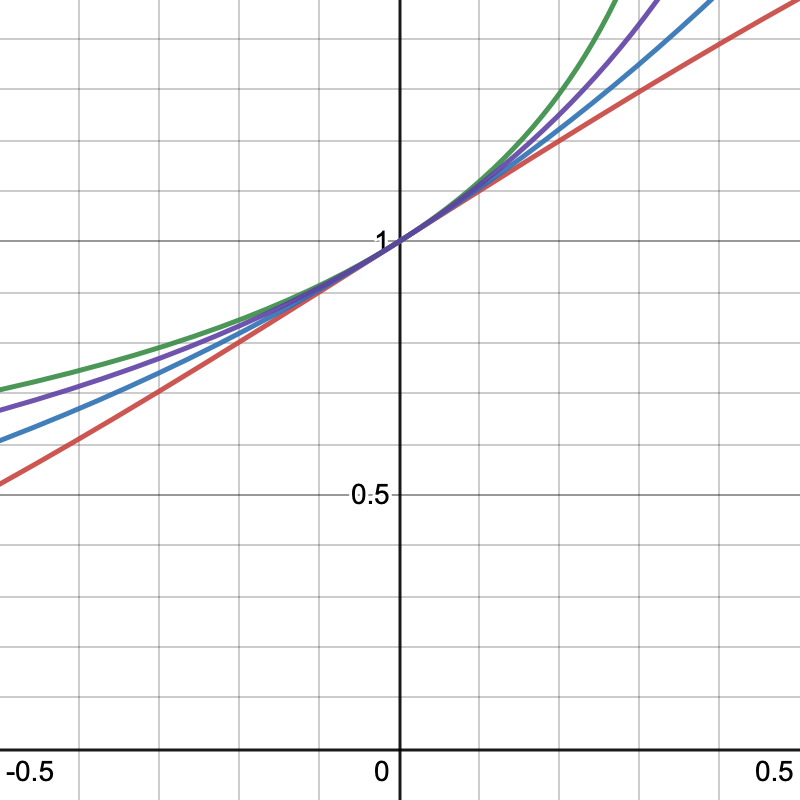
\includegraphics[width=6cm]{pic/fourtayapprox.png}
\anngraphics{6cm}{pic/fourtayapprox.png}{Graphs of $1+sin(x)$, $exp(x)$,
$\frac{1}{\sqrt{1-2x}}, and $\frac{1}{1-x}$ are plotted on a coordinate
plane. While all intersect at the point $(0,1)$, their varying curvatures
result in slightly different-looking functions.}
\end{center}
\caption{Four close functions}
\label{figfourtayapprox}
\end{figure}
All four have value $1$ at $0$ and increase, in a plot
(Figure~\ref{figfourtayapprox}, deliberately not labeled)
they are close for small values of $\sz{x}$. It seems hard to determine by
hand which graph belongs to which function.

To help with this decision, consider Taylor approximations of the four
functions:
\[
\begin{array}{lrcl}
\mbox{a)}&  1+\sin(x)&\sim&{\displaystyle%
1+x-\frac{x^3}{6}+\frac{x^5}{120}-\frac{x^7}{5040}+\cdots}\\
\\
\mbox{b)}&  \exp(x)&\sim&{\displaystyle%
1+x+\frac{x^2}{2}+\frac{x^3}{6}+\frac{x^4}{24}+\frac{x^5}{120}+\cdots}\\
\\
\mbox{c)}&{\displaystyle  \frac{1}{\sqrt{1-2x}}}&\sim&{\displaystyle%
1+x+\frac{3x^2}{2}+\frac{5x^3}{2}+\frac{35x^4}{8}+\frac{63x^5}{8}+\cdots}\\
\\
\mbox{d)}&{\displaystyle  \frac{1}{1-x}}&\sim&{\displaystyle%
1+x+x^2+x^3+x^4+x^5+\cdots}\\
\end{array}
\]
All start with $1+x$, which explains why the functions are so close for
small $\sz{x}$. But the coefficients of the $x^2$ terms differ, they are (in
increasing order) $0$ for a), $\frac12$ for b), $1$ for d) and $\frac32$ for
c). This means that for small values of $x$, we expect $1+\sin(x)$ to be the
smallest and $\frac{1}{\sqrt{1-2x}}$ to be the largest. Since $x^2=(-x)^2$
this will hold for both positive and negative $x$, as the plot shows.
And for $\sz{x}$ sufficiently small the graph of $1+x+\frac34x^2$
would\mynote{not depicted in the plot as this requires serious zooming in for
negative $x$.} lie in the middle between the top and bottom two lines.


\subsection{Using the error estimate}

We briefly illustrate how the error term formula can be used to get a
concrete estimate of the approximation error. Suppose we
want to approximate $\sin(x)$ on the interval from $-2$ to $2$ by a Taylor
polynomial, centered at $a=0$. Then (because of the interval) $\sz{x-a}\le
2$. Next we want to estimate the derivatives. Since $\ddx{x}\sin(x)=\cos(x)$
and $\ddx{x}\cos{x}=-\sin(x)$ we choose $M=1$ as the largest value of these
functions. (We could have chosen also $M=5$ as a (not that tight) bound. In
other cases it can be harder to give very tight estimates, but usually even
a rough estimate will usually do well. The error estimate then gives us an
error
\[
\sz{f(x)-p_3(x)}\le \frac{1}{4!}2^4\sim 0.66
\]
for a polynomial of degree $3$.
\mynote{Note that this is an estimate and a promise that the error is not worse.
Actually the error typically will be much smaller than what the estimate.}
For a degree 8 approximation \mynote{For $f(x)=\sin(x)$ the degree 8 Taylor
polynomial is actually the same as the degree 7 Taylor polynomial.}
\[
\sz{f(x)-p_8(x)}\le \frac{1}{9!}2^9=\frac{512}{362880}\sim 0.0014.
\]
If we wanted to guarantee an error of less than $10^{-6}$ we can try out
increasing values for $n$ \mynote{since solving the equation for $n$ is
not possible} and find that this is the case for $n\ge 14$.
\smallskip

An somewhat obvious improvement of the approximation is by cranking up the
degree. Basically, we shall show in Section~\ref{sectaylors}
that a Taylor polynomial ``of degree
infinity'' can be used in place of the function (with exact values, no
approximation).

\subsection{Fast inverse square root}

%TN rewrite AH
An application of Taylor approximations together with Newton's Method 
is found in a famous example of an
optimized routine, namely the evaluation of the function $a\mapsto
\frac{1}{\sqrt(a)}$.

This function is used in digital signal processing to re-scale a vector to
length 1, which is required for example when calculating the illumination
level and shading of a surface in 3D graphics. 

When rendering a scene, this value has to be calculated separately for each
triangle, its execution therefore is highly time critical.

While the newer x86 SSE instruction set includes a dedicated operation
\texttt{rsqrtss} for it, historically this functionality had to be coded from
more basic operations. However both square root and division are expensive,
which explains why other approaches have been considered.

The following method became prominent in the early 2000s as being used in
the video game \texttt{Quake III}, though it dates back to uses in computer
graphics in the 1980s, for example on \texttt{SGI Indigo} graphics
workstations. What we shall describe is a somewhat simplified version, that
leaves out subtleties in how numbers are coded on the computer\footnote{this
incidentally is also the
reason for the name ``\texttt{0x5F3759DF} method'' that is sometimes used},
and how error is minimized.
\medskip

The method works by first computing one rough approximation of the value,
and then using one step of the Newton method to refine the result. (It turns
out that the initial approximation is good enough that one step of the
Newton method suffices, but we shall not show this.)
\smallskip

\begin{bsp}
The input number $a$ (when computing $1/\sqrt{a}$)
is given as a floating point number in the form\mynote{This is dictated by
the CPU of the computer}
\[
a=2^e\cdot(1+m)
\]
with $0\le m<1$ (if we had $m>1$ one could instead increase $e$).
That means that
\[
\frac{1}{\sqrt{a}}=2^{-\frac12e}\cdot\frac{1}{\sqrt{1+m}}.
\]
The term $2^{-\frac12e}$ can immediately be taken as a factor of a power of
$2$. For the second factor we look at the Taylor polynomial (with respect to
the variable $m$) for $\frac{1}{\sqrt{1+m}}$, which is 
\[
1-\frac{m}{2}+\frac{3m^2}{8}+\cdots
\]
and use the degree 1 approximation $1-\frac{m}{2}$. (Here in fact, the
code uses a number different from $1$ to minimize the error, but
how this is done is beyond the scope of this text.) Note that $m/2$ can be
computed cheaply as a shift of a binary number.

We thus have the initial approximation 
\[
a_0=2^{-\frac12e}\cdot\left(1-\frac{m}2\right).
\]

Now for the Newton method. The function we want to find a zero of is 
\[
f(x)=\frac{1}{x^2}-a,
\]
whose value will be zero exactly when
$x=\frac1{\sqrt{x}}$. Newton's method (Section~\ref{secnewton}) states that
the next iteration must be
\[
a_{n+1}=a_n-\frac{f(a_n)}{f'(a_n}).
\]
We calculate $f'(x)=-\frac{2}{x^3}$ and thus
\[
\frac{f(x)}{f'(x)}=\frac{\frac{1-x^2a}{x^2}}{-\frac{2}{x^3}}
=\frac{x(1-ax^2)}{2}.
\]
The first Newton iterate is thus
\[
a_1=a_0+\frac{a_0(1-a_0x^2)}{2}
=\frac{a_0(3-a_0x^2)}{2}=a_0\left(\frac{3}{2}-\frac{a}{2}a_0^2\right).
\]
This gives us the algorithm (as published on the web, e.g.
\url{https://en.wikipedia.org/wiki/Fast_inverse_square_root}):
\begin{verbatim}
1   const float threehalfs = 1.5F;

2   x2= number * 0.5F;
3   y = number;
4   i  = *(long*) &y;      // floating point hacking
5   i = 0x5f3759df-(i>>1); 
6   y = * ( float * ) &i;
7   y = y * ( threehalfs - ( x2 * y * y ) ); // 1st iteration
\end{verbatim}
Lines 4-6 calculate $2^{-\frac12e}\cdot\left(c-\frac{m}2\right)$ with some
trickery that uses bit operations on floating point numbers by reinterpreting
their bit pattern as an integer -- the
\texttt{(i>>1)} is the $\frac{m}{2}$ and the hexadecimal constant is the
optimized value for $c$.
Line 7 then is the Newton iteration. (The code in fact includes a second
iteration that has been commented out, as the first one turned out to be good
enough in practice.)
\end{bsp}

\section{Taylor Series}
\label{sectaylors}

If we form Taylor polynomials of increasing degree for a function $f(x)$
(that is infinitely often differentiable),
we get a sequence of partial sums of the infinite
\defini{Taylor Series}\mynote{For
reasons of time we now focus only on the case of series centered around
$a=0$. The same theory would hold if we center around another $a$ and
replace $x$ by $x-a$.}
\[
t(x)=\sum_{i=0}^\infty\frac{f^{(i)}(0)}{i!} x^i.
\]
While it might look strange to have the variable $x$ involved, one could
imagine setting $x$ to some number, then this becomes just an ordinary
series. We call such series, that involve powers of a variable $x$,
\defini{power series}.

For example, we get for $f(x)=\exp(x)$ the Taylor series
\[
t(x)=\sum_{i=0}^\infty\frac{1}{i!} x^i.
\]

One can show that for such a series there exists $b\ge 0$ such that:
\begin{itemize}
\item[a)]
The
series converges, if $-b<x<b$.
\item[b)]
If $-b<x<b$ one has that $f(x)=t(x)$ (where $t(x)$ is the limit of the
infinite series for the chosen value $x$.
\item[c)] If there is {\em any} power series with properties a) and b) that
produces the values of $f$, it must be identical to $t(x)$.
\end{itemize}
The actual value of $b$ will depend on the
coefficients (and thus on the function $f$), or one can describe it using
the error term from the previous section.
In bad cases it can be just $0$, but there are many important functions for
which $b$ can be chosen arbitrary large. (Such functions are called
\defini{analytic}.)
\medskip

These facts have a number of important consequences, which we shall briefly
explore:
\paragraph{Treating Functions as if they are Polynomials:}
We shall see below that such power series can be treated, for arithmetic, as
well as for calculating derivatives, as if they were polynomials (albeit of
infinite degree). This can make some arguments about such functions easier.

\paragraph{Finding Taylor polynomials and Taylor series:} Taylor polynomials are just partial
sums of Taylor series. We shall see that we can manipulate Taylor series to
obtain series for functions for which it would be harder to find Taylor
polynomials by direct means (that is calculating derivatives).

\paragraph{Defining new functions:} A very convenient way of defining
functions with particular properties is as Taylor series. Indeed, this is
how functions such as $\exp(x)$ and $\sin(x)$ get properly defined: The
definition in school, as powers $e^x$ or ratios of sides of triangles, cause
difficulties\mynote{Not to say they actually never address the question!}
in how one would evaluate these for irrational values of $x$.

Instead, mathematicians {\em define} these functions through power series

\begin{eqnarray*}
\exp(x)&=&\sum_{i=0}^\infty\frac{1}{i!} x^i\\
\sin(x)&=&\sum_{i=0}^\infty
\frac{(-1)^i}{(2i+1)!}x^{2i+1}=x-\frac{x^3}{3!}+\frac{x^5}{5!}-\cdots
\end{eqnarray*}
and then show that these functions agree with (and have the same properties)
as the functions with the same names known from school.
\smallskip

There are many other functions (for example so-called ``Bessel functions'')
that arise in applications of mathematics, and that are only defined as such
a Taylor series.

\subsection{Complex Numbers}

Taylor series thus also are the key of extending the definition of functions to
the complex numbers. Being based on polynomials, one can evaluate a Taylor
series at a complex number as well as one could do at a real number. This
makes it possible to define (say) $\sin(x)$ for a complex value of $x$, even
though the geometric interpretation then does not make sense.

We illustrate this in a classical example, that is called \defini{Euler's
formula}, which connects the exponential function with sine and cosine: Substitute $ix$ (where $i^2=-1$)
for $x$ in the exponential function, and we get
\begin{eqnarray*}
 e^{ix} &=& 1 + ix + \frac{(ix)^2}{2!} + \frac{(ix)^3}{3!} + \frac{(ix)^4}{4!} + \frac{(ix)^5}{5!} + \frac{(ix)^6}{6!} + \frac{(ix)^7}{7!} + \frac{(ix)^8}{8!} + \cdots \\
 &=& 1 + ix - \frac{x^2}{2!} - \frac{ix^3}{3!} + \frac{x^4}{4!} + \frac{ix^5}{5!} - \frac{x^6}{6!} - \frac{ix^7}{7!} + \frac{x^8}{8!} + \cdots \\
 &=& \left( 1 - \frac{x^2}{2!} + \frac{x^4}{4!} - \frac{x^6}{6!} + \frac{x^8}{8!} - \cdots \right) + i\left( x - \frac{x^3}{3!} + \frac{x^5}{5!} - \frac{x^7}{7!} + \cdots \right) \\
 &=& \cos(x) + i\sin(x) ,
\end{eqnarray*}
and thus in particular that
\[
1+e^{i\cdot\pi}=0.
\]
Evaluating also $e^{-ix}$ allows us to solve for $\sin(x)$ and $\cos(x)$ and
express both functions in terms of the exponential function as
\begin{eqnarray*}
\sin x &= \operatorname{Im} \left(e^{ix}\right) =\frac{e^{ix} - e^{-ix}}{2i},\\
\cos x &= \operatorname{Re} \left(e^{ix}\right) =\frac{e^{ix} + e^{-ix}}{2}.
\end{eqnarray*}

\subsection{Taylor Series Operations}

Before looking at (and constructing) more examples, we briefly state some
of the properties for arithmetic with Taylor series. The basic rule is that
in the interval of convergence, Taylor series behave like polynomials:

\begin{thm}
Let $f,g\colon\R \to\R$ be functions that are infinitely often differentiable
and that are (for values of $x$ in a given interval) equal to their
respective Taylor series
\[
f(x)=\sum_{i=0}^\infty a_i x^i,\quad
g(x)=\sum_{i=0}^\infty b_i x^i.
\]
Then (for values of $x$ in the interval) we have that
\begin{enumerate}
\item For $c\in R$, $(cf)(x)=\sum_{i=0}^\infty (c\cdot a_i)x^i$.
\item $(f+g)(x)=f(x)+g(x)=\sum_{i=0}^\infty (a_i+b_i) x^i$.
\item $(f\cdot g)(x)=f(x)\cdot g(x)=\sum_{i=0}^\infty \left(\sum_{j=0}^i
a_j\cdot b_{i-j}\right) x^i$.
\item $f'(x)=\sum_{i=0}^\infty (i+1)a_{i+1}x^i
=\sum_{i=1}^\infty i\cdot a_i x^{i-1}$.
\item The power series $F(x)=\sum_{i=0}^\infty \frac{a_i}{i+1} x^{i+1}$ has
the derivative $F'(x)=f(x)$. (I.e. $F$ is an {\em antiderivative} of $f$.)
\end{enumerate}
In summary, Taylor series can be treated like polynomials.
\end{thm}
Note that -- since Taylor series are unique -- these equations give {\em the}
Taylor series for the respective functions, and any operation (such as
substituting $x^k$ for $x$) on a Taylor series must be the Taylor series for
the same operation of a function.
\medskip

As with polynomials, if a function is even (that is $f(x)=f(-x)$) then all
powers of $x$ in the Taylor series have even exponent. Similarly all
powers have odd exponent, if the function is odd ($f(-x)=-f(x)$).

\subsection{Examples and Applications}

This theorem has interesting consequences for finding derivatives and Taylor
series.

Let us start with the Taylor series for $\exp(x)$ which is (for any
$x\in\R$)
\[
\exp(x)=\sum_{i=0}^\infty \frac{1}{i!} x^i.
\]
Its derivative thus is
\[
\frac{\mbox{d}}{\mbox{d}x}
\exp(x)=\sum_{i=0}^\infty \frac{i+1}{(i+1)!} x^i
=\sum_{i=0}^\infty \frac{i}{i!} x^i=\exp(x).
\]
This proves that $\frac{\mbox{d}}{\mbox{d}x}\exp(x)=\exp(x)$.
\smallskip

Similarly, consider the Taylor series for $\sin(x)$ which is
\[
\sin(x)=\sum_{i=0}^\infty
\frac{(-1)^i}{(2i+1)!}x^{2i+1}=x-\frac{x^3}{3!}+\frac{x^5}{5!}-\cdots
\]
We thus have the derivative
\[
\frac{\mbox{d}}{\mbox{d}x}
\sin(x)=
1-\frac{x^2}{2!}+\frac{x^4}{4!}-\cdots
=\sum_{i=0}^\infty \frac{(-1)^{i+1}}{(2i)!}x^{2i}=\cos(x)
\]
(and similarly for the derivative of $\cos(x)$.)

{\em These observations are ultimately the
justifications for the derivatives of elementary functions we stated in
Section~\ref{derelem}.}
\smallskip

Next, if $\sz{x}<1$ the formula for the geometric series gives us that
\[
\frac{1}{1-x}=1+x+x^2+x^3+\cdots=\sum_{i=0}^\infty x^i
\]
Substituting $-x$ for $x$ gives us
\[
\frac{1}{1+x}=\sum_{i=0}^\infty (-1)^i x^i
\]
We know that $F(x)=\log(1+x)$ is a function with $F'(x)=1/(1+x)$ and
$F(0)=0$. We thus get the new Taylor series
\[
\log(1+x)=x-\frac{x^2}{2}+\frac{x^3}{3}-\cdots=\sum_{i=1}^\infty\frac{(-1)^{i+1}}{i}x^i.
\]
\smallskip

Returning to the use of the geometric series, we can write
\[
\frac{x}{x-3}=-\frac{x}{3}\frac{1}{1-x/3}.
\]
Substituting $x/3$ into the series for $\frac{1}{1-x}$ gives us
\[
\frac{1}{1-x/3}=-\sum_{i=0}^\infty \left(\frac{x}{3}\right)^i,
\]
and thus
\[
\frac{x}{x-3}= -\frac{x}{3}\sum_{i=0}^\infty \left(\frac{x}{3}\right)^i
= \sum_{i=1}^\infty \left(\frac{x}{3}\right)^i.
\]
One can use this idea more generally (this goes under the name of
\defini{partial fractions}, but we won't go into details here) for rational
functions, that is fractions of polynomials. If we can write these as sums
of fractions with easier denominators (that is, factors of the original
denominator), it is possible to combine Taylor series of the summands to a
series for the original function.

For example (You should be able to follow this calculation, but it is not
expected that you would be able to come up with it on your own), consider
\[
f(x)=\frac{21x-15}{x^3-7x^2+5x-35}=\frac{-3x}{x^2+5}+\frac{3}{x-7}.
\]
As above, we calculate
\[
\frac{3}{x-7}=-\frac{3}{7}\frac{1}{1-x/7}=-\frac{3}{7}
\sum_{i=0}^\infty \left(\frac{x}{7}\right)^i
=\sum_{i=0}^\infty \frac{-3x^i}{7^{i+1}}.
\]
and
\[
\frac{-3x}{x^2+5}=\frac{3x}{5}\frac{1}{1-(-x^2/5)}=\frac{3x}{5}
\sum_{i=0}^\infty \left(\frac{-x^2}{5}\right)^i
=-\frac{3x}{5}
+\frac{3x^3}{25}
-\frac{3x^5}{125}+\cdots,
\]
combining to a Taylor series for $f(x)$:
\begin{eqnarray*}
\frac{21x-15}{x^3-7x^2+5x-35}&=&
\frac{3}{7}-\frac{132 x}{245}-\frac{279 x^{2}}{1715}+\frac{5808
x^{3}}{60025}+\frac{13011 x^{4}}{420175}-\frac{287892 x^{5}}{14706125}\\
&&-\frac{640839 x^{6}}{102942875}+\frac{14090208 x^{7}}{3603000625}
+\frac{31384611 x^{8}}{25221004375}\\
&&-\frac{690502692 x^{9}}{882735153125}-
x\frac{1537928439 x^{10}}{6179146071875}
%+\frac{33834219408 x^{11}}{216270112515625}+\frac{75358081011 x^{12}}{1513890787609375}
+\cdots
\end{eqnarray*}

%More elaborate manipulations are possible. For example we have (we will see
%this in the homework) that the Taylor series for $\arctan(x)$ is:
%\[
%x-\frac{x^3}{3}+\frac{x^5}{5}-\frac{x^7}{7}+\cdots
%\]
%If we use that 

\section{Outlook: Solving Recursions}
\label{solvfibo}

A powerful mathematical tool, called \defini{generating functions} uses
Taylor series manipulations to find explicit expressions for recursively
defined series. 

We illustrate this with the example of the Fibonacci
numbers, defined as:
\[
f_0=0,\qquad f_1=1,\qquad f_{n+2}=f_{n+1}+f_n.
\]
We now define a function from a Taylor series, whose coefficients are the
Fibonacci numbers:
\[
F(x)=\sum_{i=0}^\infty f_i x^i=x+x^2+2x^3+3x^4+5x^5+8x^6+13x^7+\cdots
\]
Note that
\[
xF(x)=\sum_{i=0}^\infty f_i x^{i+1}=\sum_{i=1}^\infty f_{i-1} x^i
\]
and
\[
x^2F(x)=\sum_{i=0}^\infty f_i x^{i+2}=\sum_{i=2}^\infty f_{i-2} x^i
\]
and thus
\begin{eqnarray*}
xF(x)+x^2F(x)&=&f_0x+\sum_{i=2}^\infty \underbrace{(f_{i-1}+f_{i-2})}_{=f_i} x^i
=\sum_{i=2}^\infty f_i x^i\\
&=&\sum_{i=0}^\infty f_i x^i-f_0-f_1x=F(x)-x.
\end{eqnarray*}
We can solve this equation for $F(x)$, and get
\[
F(x)=\frac{x}{1-x-x^2}=x\cdot\left(\frac{a}{x-\alpha}+\frac{b}{x-\beta}\right)
\]
for
\[
\alpha=\frac{-1+\sqrt{5}}{2},\quad\beta=\frac{-1-\sqrt{5}}{2},\quad
a=\frac{-1}{\sqrt{5}},\quad b=\frac{1}{\sqrt{5}}.
\]
The geometric series gives us (as above) that 
\[
\frac{a}{x-\alpha}=\sum_{i=0}^\infty \frac{-a}{\alpha^{i+1}}x^i,\quad
\frac{b}{x-\beta}=\sum_{i=0}^\infty \frac{-b}{\beta^{i+1}}x^i,
\]
and thus the Taylor series
\begin{eqnarray*}
F(x)&=& x\cdot
\sum_{i=0}^\infty\left(\frac{-a}{\alpha^{i+1}}+\frac{-b}{\beta^{i+1}}\right)x^i\\
&=&
\sum_{i=0}^\infty\left(\frac{-a}{\alpha^{i+1}}+\frac{-b}{\beta^{i+1}}\right)x^{i+1}
=\sum_{i=1}^\infty\left(\frac{-a}{\alpha^{i}}+\frac{-b}{\beta^{i}}\right)x^{i}.
\end{eqnarray*}
Comparing the coefficients of $x^i$ (which we can do because Taylor series
are unique) gives us that for $i>0$ we have
\begin{eqnarray*}
f_i&=&\frac{-a}{\alpha^{i}}+\frac{-b}{\beta^{i}}
=
\frac{1}{\sqrt{5}\cdot \alpha^i}+\frac{-1}{\sqrt{5}\cdot \beta^i}\\
&=&
\frac{1}{\sqrt{5}\cdot \left(\frac{-1+\sqrt{5}}{2}\right)^i}
+\frac{-1}{\sqrt{5}\cdot \left(\frac{-1-\sqrt{5}}{2}\right)^i}\\
&=&\frac{1}{\sqrt{5}}\left(\left(\frac{2}{\sqrt{5}-1}\right)^i+\left(\frac{2}{\sqrt{5}+1}\right)^i\right),
\end{eqnarray*}
which is an explicit formula for the Fibonacci numbers.
